\typeout{NT FILE chapter-rs232-interface.tex}%
\chapter{RS-232 Interface}
\label{cha:rs232-interface}

This chapter describes the \gls{rs232-interface} developed during this work. It
begins with a brief introduction to the \gls{RS232} standard, followed by a
description of the objectives, design, and implementation of the interface.

\section{RS-232 Standard}

\gls{RS232} is a standard for serial communication that defines the electrical
characteristics of the signals used in a point-to-point communication system
between a single transmitter and a single receiver. It is widely used in
industrial and laboratory instrumentation due to its simplicity, reliability,
and broad hardware support.\cite{wikipediaRS232}

The standard uses single-ended signalling referenced to a common ground, with
logic levels defined between $\pm$3\,V and $\pm$15\,V, providing adequate noise
immunity for the cable lengths typically encountered in laboratory and
industrial environments. The maximum specified cable length is 15\,m at the
standard's nominal data rate, though in practice longer cables are commonly
used at lower baud rates. Typical baud rates range from 9600 to 115200\,bps,
which is sufficient for command and status exchange in instrumentation
applications.

\section{Objective and Motivation}

The \gls{GNSS} signal generation system developed in this work must be
controllable by a remote controller or computer, which issues commands and
receives status information at runtime. \gls{RS232} was selected as the
physical communication channel for this purpose, given its ubiquity in
instrumentation environments and the straightforward point-to-point topology it
provides.

Beyond this general suitability, the choice of \gls{RS232} was in practice
dictated by an external constraint: the system needed to be integrated with
legacy equipment that communicates exclusively over \gls{RS232}. Modifying or
replacing that equipment's communication interface was outside the scope of
this internship. It should be noted that the original internship proposal
referred to \gls{RS485} instead of \gls{RS232}; as discussed in
\autoref{sec:scope-evolution}, this was a misnomer in the proposal document
rather than an intentional design choice, and \gls{RS232} was the protocol
required from the outset. RS-232 was therefore not purely a design preference,
but a constraint imposed by the pre-existing environment the system had to
integrate with.

The objective of the \gls{rs232-interface} is therefore not to define yet
another command protocol, but to turn the available serial connection into a
standards-based transport that higher-level software can reuse. In the final
architecture, \gls{RS232} carries \gls{PPP}, which creates a point-to-point IP
link between the communicating systems. Once that link is established, the
existing gRPC control interface can operate unchanged over ordinary sockets.

This approach has two main advantages. First, it removes the need to maintain
a second application-layer protocol alongside gRPC. Second, it allows standard
networking and debugging tools to be reused, making the serial integration path
behave much more like any other IP-based deployment.

\section{Design and Implementation}

The \gls{rs232-interface} was implemented as a layered transport path. At the
lowest level, the serial device is configured with the required electrical and
\texttt{termios} parameters. On top of that, \gls{PPP} is established to
encapsulate IP packets over the serial byte stream. Once the link is active,
the communicating peers exchange traffic using ordinary IP networking, and the
gRPC client and server operate above that layer without requiring any
serial-specific application logic.

This design intentionally delegates framing, packet integrity, and network
bring-up to mature, well-understood protocol layers instead of reimplementing
those concerns in project-specific code. The \gls{RS232} component therefore
focuses on link establishment, peer configuration, and operational reliability
rather than on custom message parsing.

In line with the design choices made in the \gls{sdr-control-system}, the
\gls{rs232-interface} uses errors as values rather than exceptions, and the
surrounding project is built with CMake.\cite{cmake} The resulting solution was
kept deliberately small: once the serial and \gls{PPP} layers are configured
correctly, higher-level behaviour is almost entirely inherited from the already
existing IP and gRPC stack.

\section{Architecture Diagram}

Diagram~\ref{fig:rs232-interface-architecture} illustrates the architecture of
the \gls{rs232-interface}. The serial device driver provides access to the
physical \gls{RS232} link. Above it, a \gls{PPP} endpoint encapsulates and
decapsulates IP packets. The IP layer then exposes an ordinary network
interface to the gRPC client and server, allowing the same application
protocols used on other network transports to be reused unchanged.

\begin{figure}[htbp]
      \centering
      \usetikzlibrary{positioning, fit, backgrounds, arrows.meta, calc}

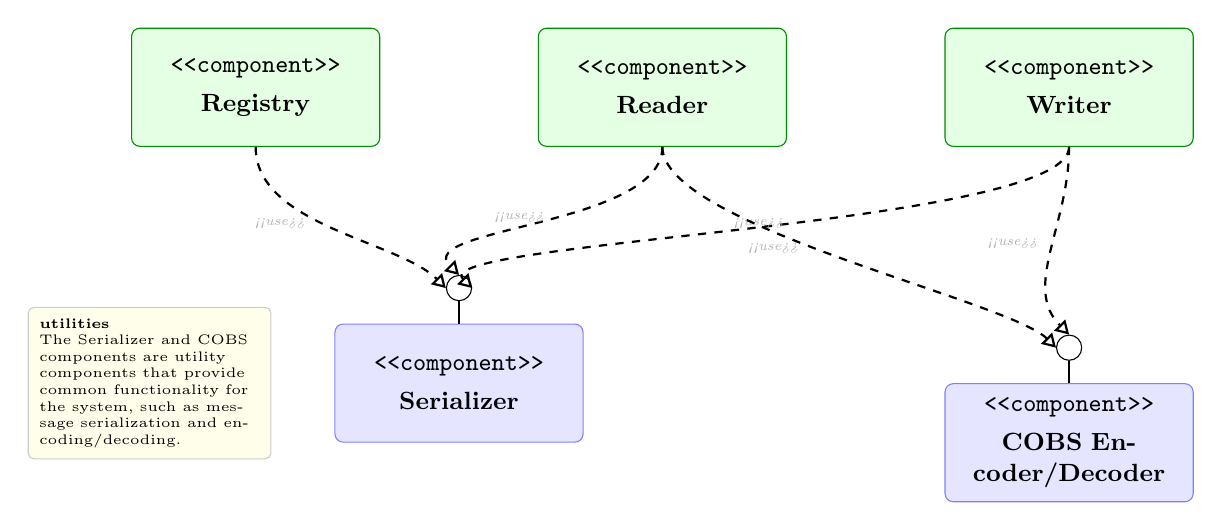
\begin{tikzpicture}[
    % ── node styles ─────────────────────────────────────────
    comp/.style = { draw, rounded corners=3pt, minimum width=3.0cm, minimum
            height=1.5cm, text width=2.8cm, align=center, font=\small, inner sep=5pt, },
    lollipop/.style = { draw, circle, minimum size=0.32cm, inner sep=0pt,
            fill=white, }, stereo/.style = {font=\tiny\itshape, text=gray!60}, use/.style =
    {->, >={Triangle[open]}, dashed, thick}, realize/.style = {->,
    >={Triangle[open]}, dashed, thick, double distance=1.2pt}, assoc/.style =
        {thick}, note/.style = { draw=gray!40, fill=yellow!8, rounded corners=2pt,
            font=\tiny, text width=2.8cm, align=left, inner sep=4pt, }, node distance =
    1.4cm, ]

    % ============================================================
    % ROW 1 — Registry  |  Reader |  Writer
    % ============================================================
    \node[comp, fill=green!10, draw=green!55!black]
    (registry) at (0,0)
    {\texttt{<<component>>}\\[3pt]\textbf{Registry}};

    \node[comp, fill=green!10, draw=green!55!black,
        right=2.0cm of registry]
    (reader)
    {\texttt{<<component>>}\\[3pt]\textbf{Reader}};

    \node[comp, fill=green!10, draw=green!55!black,
        right=2.0cm of reader]
    (writer)
    {\texttt{<<component>>}\\[3pt]\textbf{Writer}};

    % ============================================================
    % ROW 2 — Serializer  |  COBS
    % ============================================================
    \node[comp, fill=blue!10, draw=blue!50,
        below=3.0cm of $(registry)!0.5!(reader)$]
    (serializer)
    {\texttt{<<component>>}\\[3pt]\textbf{Serializer}};
    \node[comp, fill=blue!10, draw=blue!50,
        below=3.0cm of writer]
    (cobs)
    {\texttt{<<component>>}\\[3pt]\textbf{COBS Encoder/Decoder}};

    % ============================================================
    % ROW 3 — DTAPI
    % ============================================================

    % ============================================================
    % ROW 4 — Hardware
    % ============================================================

    % ============================================================
    % PROVIDED INTERFACE LOLLIPOPS
    % ============================================================
    \node[lollipop](serializer-lollipop) at ($(serializer.north)+(0,0.45)$){};
    \node[lollipop](cobs-lollipop) at ($(cobs.north)+(0,0.45)$){};

    \draw[assoc] (serializer.north) -- (serializer-lollipop);
    \draw[assoc] (cobs.north) -- (cobs-lollipop);

    % ============================================================
    % DEPENDENCY ARROWS
    % ============================================================
    % Registry --<<use>>--> Serializer
    \draw[use]
    (registry.south) .. controls +(0,-1.0) and +(-0.6, 0.6) .. (serializer-lollipop.west)
    node[stereo, pos=0.45, left=2pt] {<<use>>};
    \draw[use]
    (reader.south) .. controls +(0,-1.0) and +(-0.6, 0.6) .. (serializer-lollipop.north)
    node[stereo, pos=0.45, left=2pt] {<<use>>};
    \draw[use]
    (writer.south) .. controls +(0,-1.0) and +(-0.6, 0.6) .. (serializer-lollipop.east)
    node[stereo, pos=0.45, left=2pt] {<<use>>};

    \draw[use]
    (reader.south) .. controls +(0,-1.0) and +(-0.6, 0.6) .. (cobs-lollipop.west)
    node[stereo, pos=0.45, left=2pt] {<<use>>};
    \draw[use]
    (writer.south) .. controls +(0,-1.0) and +(-0.6, 0.6) .. (cobs-lollipop.north)
    node[stereo, pos=0.45, left=2pt] {<<use>>};

    % ============================================================
    % ANNOTATION NOTE
    % ============================================================
    \node[note, left=0.8cm of serializer] (note-utility) {
        \textbf{utilities}\\
        The Serializer and COBS components are utility components that provide
        common functionality for the system, such as message serialization and
        encoding/decoding.
    };

\end{tikzpicture}
      \caption{RS-232 Interface Architecture}
      \label{fig:rs232-interface-architecture}
\end{figure}

\section{Functionality and Use Cases}

The \gls{rs232-interface} provides the following core functionalities:

\begin{itemize}
      \item \textbf{Serial link configuration:} the interface configures and
            validates the \gls{RS232} channel used by the communicating peers.
      \item \textbf{\gls{PPP} link establishment:} the interface brings up a
            point-to-point IP connection over the serial medium.
      \item \textbf{IP transport for control traffic:} once the link is active,
            control and status messages flow as ordinary network traffic rather
            than through a bespoke serial protocol.
      \item \textbf{Reuse of the gRPC control plane:} the same gRPC contract
            used elsewhere in the system can be transported through the
            resulting IP channel without modification.
\end{itemize}

A typical use case involves a remote controller establishing the \gls{PPP} link
over \gls{RS232}, obtaining reachability to the generator through the resulting
point-to-point network interface, and then issuing gRPC requests to the control
service. From the perspective of the application layer, the interaction is the
same as on any other IP network; the fact that the underlying transport is a
serial link is largely hidden below the network layer.
